\documentclass[10pt,a4paper]{article}


%% TODO: add a question illustrating ill-conditioning.
%% Can e.g. be done using the matrix in question 1 by letting
%% x's to nearly coincide and perturbing y's a little bit.


\usepackage[english]{babel}

\usepackage[margin=22mm]{geometry}
\usepackage{amsmath,amsthm,amssymb,scrextend,graphicx,ifthen,hyperref}
\usepackage{fancyhdr}
\usepackage{mathtools}
\pagestyle{fancy}

\usepackage{algorithmic}
%\usepackage{algpseudocode}
\usepackage{mdframed}

\usepackage{tcolorbox}
\usepackage{tikz}
\usepackage{todonotes}

\usepackage{pgfplots,pgfplotstable}
\pgfplotsset{compat=1.15}

\usepackage[small,compact]{titlesec}
\titlespacing{\section}{0pt}{2ex}{1ex}
\titlespacing{\subsection}{0pt}{1ex}{0ex}
\titlespacing{\subsubsection}{0pt}{0.5ex}{0ex}
\setlength{\parskip}{0cm}
\setlength{\parindent}{1em}


\newcommand{\N}{\mathbb{N}}
\newcommand{\Z}{\mathbb{Z}}
\newcommand{\I}{\mathbb{I}}
\newcommand{\R}{\mathbb{R}}
\newcommand{\F}{\mathbb{F}}
\newcommand{\C}{\mathbb{C}}
\newcommand{\Q}{\mathbb{Q}}
\renewcommand{\qed}{\hfill$\blacksquare$}
\renewcommand{\Re}{Re}
\let\newproof\proof
\renewenvironment{proof}{\begin{addmargin}[1em]{0em}\begin{newproof}}{\end{newproof}\end{addmargin}\qed}
% \newcommand{\expl}[1]{\text{\hfill[#1]}$}

\theoremstyle{plain}
\newtheorem{theorem}{Theorem}
\newtheorem{proposition}[theorem]{Proposition}
\newtheorem{lemma}[theorem]{Lemma}
\newtheorem{corollary}[theorem]{Corollary}
\newtheorem{claim}[theorem]{Claim}
\newtheorem{problem}{Problem}

\theoremstyle{definition}
\newtheorem{definition}[theorem]{Definition}
\newtheorem{example}[theorem]{Example}
%\newtheorem*{comment}{Comment}

\newtheorem{remark}[theorem]{Remark}

\DeclareMathOperator{\vc}{vec}
\DeclareMathOperator{\epi}{epi}
\DeclareMathOperator{\Span}{span}
\DeclareMathOperator{\Range}{range}
\DeclareMathOperator{\Null}{null}
\DeclareMathOperator{\argmin}{arg\,min}


\newcommand{\eps}{\varepsilon}
%%% Norms etc.
\newcommand{\inner}[3][n]{\SwitchBracketsizeLeft{#1}\LeftBracketSize\langle#2,#3\SwitchBracketsizeRight{#1}\RightBracketSize\rangle}
\newcommand{\abs}[2][n]{\SwitchBracketsizeLeft{#1}\LeftBracketSize\lvert#2\SwitchBracketsizeRight{#1}\RightBracketSize\rvert}
\newcommand{\norm}[2][n]{\SwitchBracketsizeLeft{#1}\LeftBracketSize\lVert#2\SwitchBracketsizeRight{#1}\RightBracketSize\rVert}
\newcommand{\set}[3][b]{\SwitchBracketsizeLeft{#1}\LeftBracketSize\{#2:#3\SwitchBracketsizeRight{#1}\RightBracketSize\}}

\newcommand{\NextScriptStyle}[1]{{\scriptstyle{#1}}}
\newcommand{\NextScriptScriptStyle}[1]{{\scriptscriptstyle{#1}}}
\newcommand{\NextTextStyle}[1]{{\textstyle{#1}}}
\newcommand{\NextDisplayStyle}[1]{{\displaystyle{#1}}}
\newcommand{\SwitchBracketsizeLeft}[1]{
  \ifthenelse{\equal{#1}{b}\OR\equal{#1}{big}}{\let\LeftBracketSize=\bigl}{
    \ifthenelse{\equal{#1}{B}\OR\equal{#1}{Big}}{\let\LeftBracketSize=\Bigl}{
      \ifthenelse{\equal{#1}{g}\OR\equal{#1}{bigg}}{\let\LeftBracketSize=\biggl}{
    \ifthenelse{\equal{#1}{G}\OR\equal{#1}{Bigg}}{\let\LeftBracketSize=\Biggl}{
      \ifthenelse{\equal{#1}{s}\OR\equal{#1}{small}}{\let\LeftBracketSize=\NextScriptStyle}{
        \ifthenelse{\equal{#1}{ss}}{\let\LeftBracketSize=\NextScriptScriptStyle}{
          \ifthenelse{\equal{#1}{t}\OR\equal{#1}{text}}{\let\LeftBracketSize=\NextTextStyle}{
        \ifthenelse{\equal{#1}{d}\OR\equal{#1}{display}}{\let\LeftBracketSize=\NextDisplayStyle}{
          \ifthenelse{\equal{#1}{a}\OR\equal{#1}{auto}}{\let\LeftBracketSize=\left}{
            \let\LeftBracketSize=\relax}}}}}}}}}}
\newcommand{\SwitchBracketsizeRight}[1]{
  \ifthenelse{\equal{#1}{b}\OR\equal{#1}{big}}{\let\RightBracketSize=\bigr}{
    \ifthenelse{\equal{#1}{B}\OR\equal{#1}{Big}}{\let\RightBracketSize=\Bigr}{
      \ifthenelse{\equal{#1}{g}\OR\equal{#1}{bigg}}{\let\RightBracketSize=\biggr}{
    \ifthenelse{\equal{#1}{G}\OR\equal{#1}{Bigg}}{\let\RightBracketSize=\Biggr}{
      \ifthenelse{\equal{#1}{s}\OR\equal{#1}{small}}{\let\RightBracketSize=\NextScriptStyle}{
        \ifthenelse{\equal{#1}{ss}}{\let\RightBracketSize=\NextScriptScriptStyle}{
          \ifthenelse{\equal{#1}{t}\OR\equal{#1}{text}}{\let\RightBracketSize=\NextTextStyle}{
        \ifthenelse{\equal{#1}{d}\OR\equal{#1}{display}}{\let\RightBracketSize=\NextDisplayStyle}{
          \ifthenelse{\equal{#1}{a}\OR\equal{#1}{auto}}{\let\RightBracketSize=\right}{
            \let\RightBracketSize=\relax}}}}}}}}}}


\newcounter{oppgave}

\newenvironment{oppgave}[1][]{\refstepcounter{oppgave}\par\medskip
 \noindent \textbf{Question~\theoppgave. #1} \rmfamily}{\medskip}

\newcounter{punkt}[oppgave]

\newenvironment{punkt}[1][]{\refstepcounter{punkt}\par\medskip
 \noindent \textbf{\theoppgave.\thepunkt. #1} \rmfamily}{\medskip}

\newenvironment{amatrix}[1]{%
 \left[\begin{array}{@{}*{#1}{c}|c@{}}
}{%
 \end{array}\right]
}

\sloppy

\begin{document}

\lhead{SLIAL}
\chead{WS01: Linear transformations and systems of linear equations}
\rhead{\today}

\fancyfoot[R] {\thepage}
\fancyfoot[C] {}
\fancyfoot[L] {\small SEB, seb@livoni.me}
%\maketitle

\listoftodos

%------------------------------------------------------------------------
\section{Polynomial curve fitting}

Consider a dataset given by \(n\) pairs of real numbers
\[
  (t_1,y_1), (t_2,y_2), \dots, (t_n, y_n),
\]
which we interpret as \(n\) points in \(\R^2\).
We would like to find a polynomial
\[
  p(t) = q_0 + q_1 t + \dots + q_{n-1} t^{n-1},
\]
Explain why the following of degree \(n-1\), which passes through these points.
Thus we would like to solve the system of \(n\) equations
\begin{equation}\label{poly}
  \begin{aligned}
    p(t_1) &= y_1,\\
    p(t_2) &= y_2,\\
    \vdots&\\
    p(t_n) &= y_n,
  \end{aligned}
\end{equation}
for the unknown polynomial coefficients \(q = (q_0,q_1,\dots,q_{n-1})\in \R^n\).

\begin{oppgave}
  \begin{punkt}
    Write down the total matrix corresponding to the system of equations~\eqref{poly}.
  \end{punkt}
  \begin{align*}
    \begin{amatrix}{5}
      t^0_1 & t_1^1 & t_1^2 & \cdots & t_{1}^{n-1} & y_1 \\
      t^0_2 & t_2^1 & t_2^2 & \cdots & t_{2}^{n-1} & y_2 \\
      \vdots & \vdots & \vdots & \cdots & \vdots & \vdots \\
      t^0_n & t_n^1 & t_n^2 & \cdots & t_{n}^{n-1} & y_n \\ 
    \end{amatrix}
  \end{align*}

  \begin{punkt}
    Use Gaussian elimination to find the quadratic polynomial passing through the points \((1,4)\), \((2,0)\), and \((3,12)\).
    Plot the graph of the resulting polynomial and the points in the dataset.
  \end{punkt}
  \begin{gather*}
    \begin{amatrix}{3}
      1^0 & 1^1 & 1^2 & 4 \\
      2^0 & 2^1 & 2^2 & 0 \\
      3^0 & 3^1 & 3^2 & 12 \\
    \end{amatrix}
      =
      \begin{bmatrix*}[r]
      1 & 1 & 1 & 4 \\
      1 & 2 & 4 & 0 \\
      1 & 3 & 9 & 12 \\
      \end{bmatrix*}
      \sim
      \begin{bmatrix*}[r]
      1 & 1 & 1 & 4 \\
      0 & 1 & 3 & -4 \\
      0 & 2 & 8 & 8 \\
      \end{bmatrix*}
      \sim
      \begin{bmatrix*}[r]
      1 & 1 & 1 & 4 \\
      0 & 1 & 3 & -4 \\
      0 & 0 & 2 & 16 \\
      \end{bmatrix*}
      \sim
      \begin{bmatrix*}[r]
      1 & 1 & 1 & 4 \\
      0 & 1 & 3 & -4 \\
      0 & 0 & 1 & 8 \\
      \end{bmatrix*} \\
      \sim
      \begin{bmatrix*}[r]
      1 & 0 & -2 & 8 \\
      0 & 1 & 3 & -4 \\
      0 & 0 & 1 & 8 \\
      \end{bmatrix*}
      \sim
      \begin{bmatrix*}[r]
      1 & 0 & 0 & 24 \\
      0 & 1 & 3 & -4 \\
      0 & 0 & 1 & 8 \\
      \end{bmatrix*}
      \sim
      \begin{bmatrix*}[r]
      1 & 0 & 0 & 24 \\
      0 & 1 & 0 & -28 \\
      0 & 0 & 1 & 8 \\
    \end{bmatrix*}
  \end{gather*}

  After using Gaussian elimation, we cand find the coefficients being:
  \begin{align*}
    q=\begin{bmatrix*}[r]
      q_0 \\ q_1 \\ q_2
    \end{bmatrix*}
    =
    \begin{bmatrix*}[r]
      24 \\ -28 \\ 8
    \end{bmatrix*}
  \end{align*}
  %\begin{align*}
  %  q_0 \cdot 1+ q_1 \cdot 0 + q_2 \cdot 0=24 \\
  %  q_0 \cdot 0+ q_1 \cdot 1 + q_2 \cdot 0=-28 \\
  %  q_0 \cdot 0+ q_1 \cdot 0 + q_2 \cdot 1=8
  %\end{align*}

  The resulting polynomial equals to: $p(t)=q_0 +q_1 t + \dots +q_{n-1} t^{n-1}=24t^0-28t^1+8t^2$. We can plot the graph of the polynomial and points to check if the result is correct.

  \def\FunctionF(#1){24*(#1)^0 - 28*(#1)^1 + 8*(#1)^2}

  \begin{align*}
    \begin{tikzpicture}
      \begin{axis}[
            axis y line=center,
            axis x line=middle, 
            axis on top=true,
            xmin=-2,
            xmax=5.5,
            ymin=-8,
            ymax=42,
            height=8.0cm,
            width=12.0cm,
            grid,
            xtick={-2,...,5},
            ytick={-5,0,...,40},
        ]
        \addplot [domain=-5:5, samples=50, mark=none, ultra thick, blue] {\FunctionF(x)};
        \node [left, blue] at (axis cs: 3,37.5) {$24t^0-28t^1+8t^2$};
        \filldraw[blue] (1,4) circle (2pt) node[anchor=east,text=black]{(1,4)};
        \filldraw[blue] (2,0) circle (2pt) node[anchor=south,text=black]{(2,0)};
        \filldraw[blue] (3,12) circle (2pt) node[anchor=west,text=black]{(3,12)};
      \end{axis}
    \end{tikzpicture}
  \end{align*}

  And indeed it is because the three points is exactly on the line. Wuhu.

  \begin{punkt}
    Use Gaussian elimination to find the fourth degree polynomial passing through the points \((-2,3)\), \((-1,5)\), \((0,1)\), \((1,4)\), and \((2,10)\).
    Plot the graph of the resulting polynomial and the points in the dataset.
  \end{punkt}

  \begin{gather*}
    \begin{bmatrix*}[r] % [r] to make alignment with minus
      -2^0 & -2^1 & -2^2 & -2^3 & 3 \\
      -1^0 & -1^1 & -1^2 & -1^3 & 5 \\
      0^0 & 0^1 & 0^2 & 0^3 & 1 \\
      1^0 & 1^1 & 1^2 & 1^3 & 4 \\
      2^0 & 2^1 & 2^2 & 2^3 & 10
    \end{bmatrix*}
    =
    \begin{bmatrix*}[r]
      1 & -2 & 4 & -8 & 16 & 3 \\
      1 & -1 & 1 & -1 & 1 & 5 \\
      1 & 0 & 0 & 0 & 0 & 1 \\
      1 & 1 & 1 & 1 & 1 & 4 \\
      1 & 2 & 4 & 8 & 16 & 10
    \end{bmatrix*}
    \sim
    \begin{bmatrix*}[r]
      1 & 0 & 0 & 0 & 0 & 1.0000 \\
      0 & 1 & 0 & 0 & 0 & -1.2500 \\
      0 & 0 & 1 & 0 & 0 & 4.2083 \\
      0 & 0 & 0 & 1 & 0 & 0.7500 \\
      0 & 0 & 0 & 0 & 1 & -0.7083
    \end{bmatrix*} \\
    q=\begin{bmatrix*}[r]
      q_0 \\ q_1 \\ q_2 \\ q_3 \\ q_4
    \end{bmatrix*}
    =
    \begin{bmatrix*}[r]
      1.0000 \\ -1.2500 \\ 4.2083 \\ 0.7500 \\ -0.7083
    \end{bmatrix*}
  \end{gather*}

  \def\FunctionQ(#1){1*(#1)^0-1.25*(#1)^1+4.2083*(#1)^2+0.75*(#1)^3-0.7083*(#1)^4}

  \begin{align*}
    \begin{tikzpicture}
      \begin{axis}[
            axis y line=center,
            axis x line=middle, 
            axis on top=true,
            xmin=-4,
            xmax=7.5,
            ymin=-3,
            ymax=15,
            height=8.0cm,
            width=12.0cm,
            grid,
            xtick={-4,...,7},
            ytick={-2,0,...,14},
        ]
        \addplot [domain=-5:5, samples=50, mark=none, ultra thick, blue] {\FunctionQ(x)};
        \node [right, blue] at (axis cs: 0,13) {$1t^0-1.25t^1+4.2083t^2+0.75t^3-0.7083t^4$};
        \filldraw[blue] (-2,3) circle (2pt) node[anchor=east,text=black]{(-2,3)};
        \filldraw[blue] (-1,5) circle (2pt) node[anchor=west,text=black]{(-1,5)};
        \filldraw[blue] (0,1) circle (2pt) node[anchor=west,text=black]{(0,1)};
        \filldraw[blue] (1,4) circle (2pt) node[anchor=west,text=black]{(1,4)};
        \filldraw[blue] (2,10) circle (2pt) node[anchor=south,text=black]{(2,10)};
      \end{axis}
    \end{tikzpicture}
  \end{align*}

\end{oppgave}

%------------------------------------------------------------------------
\section{Linear transformations and digital image processing}

\subsection*{Digital images as vectors in \(\R^n\)}
In this workshop we will apply some of the linear algebraic concepts we learned so far towards image processing.  For simplicity, we will focus on grayscale images only.
We will think of an \(N\times M\) image \(P\) as a two-dimensional array containing \(n = NM\) real numbers representing the grayscale levels of individual pixels.\footnote{That is, we will ignore the
fact that digital images allow only a discrete number of grayscale levels.}
We can now concatenate the pixels of the image, row-by-row, in order to obtain a one-dimensional array \(v=\vc(P) \in \R^n\), see the figure below:
  \begin{tcolorbox}
    \begin{center}
\begin{tabular}{cccc}
\(2\times 3\) image: \quad
\(P=\)
\begin{tabular}{|l|c|r|}
  \hline
  \(P_{1,1}\)&\(P_{1,2}\)&\(P_{1,3}\)\\
  \hline
  \(P_{2,1}\)&\(P_{2,2}\)&\(P_{2,3}\)\\
  \hline
\end{tabular}
&
\(\iff\)
&
vector
\(
\vc(P)=
\begin{bmatrix*}[r]
  P_{1,1}\\P_{1,2}\\P_{1,3}\\P_{2,1}\\P_{2,2}\\P_{2,3}
\end{bmatrix*}
=
\begin{bmatrix*}[r]
  v_1\\v_2\\v_3\\v_4\\v_5\\v_6
\end{bmatrix*}
=v
\in \R^6
\)
\end{tabular}
\end{center}
\end{tcolorbox}
In this way the grayscale value of pixel \(P_{y,x}\), \(y=1,\dots,N\), \(x=1,\dots,M\)
corresponds to the value \(v_{M(y-1) + x}\) component in the equivalent vector representation \(v=\vc(P)\).
We will use double index notation to refer to the pixels in the image, and single index
notation to refer to the components in the vector.

\subsection*{Image convolution with a kernel}
Let \(\omega\) be a small \((2k+1) \times (2k+1)\) matrix; often \(k=1\) or \(k=2\) is used, which results in \(3\times 3\) or \(5\times 5\) matrices.
With the help of this matrix, we will now define a function (transformation) \(T\), which maps \(N \times M\) images to \(N \times M\) images.
Formally, we say that \(\vc(P)=T_\omega(\vc(O))\), when
\begin{equation}\label{eqbl}
  P_{y,x} =
  \sum_{\zeta=\max\{y-k,1\}}^{\min\{y+k,N\}}
  \sum_{\xi=\max\{x-k,1\}}^{\min\{x+k,M\}}
  \omega_{y-\zeta+k+1,x-\xi+k+1}\,
  O_{\zeta,\xi}
\end{equation}
In other words, pixels of the image \(\vc(P)=T_\omega(\vc(O))\) are weighted averages of the pixels of the image \(O\) over a small \((2k+1) \times (2k+1)\) neighbourhood,
with weights specified in the kernel matrix \(\omega\).
Below we show some examples of the application of various kernels to a small \(125\times 200\) pixel image:
\begin{center}
\begin{tabular}{lrc}
  Operation & Kernel matrix \(\omega\) & Resulting image\\
  Original image & \(\begin{bmatrix*}[r]0&0&0\\0&1&0\\0&0&0\end{bmatrix*}\)&
  \raisebox{-0.5\height}{
\includegraphics[width=0.3\textwidth]{./assets/1984_small.png}}
  \\
  Blur &
  %\(\frac{1}{16}\begin{bmatrix*}[r]1&2&1\\2&4&2\\1&2&1\end{bmatrix*}\)
  \(\frac{1}{256}\begin{bmatrix*}[r]
1 &4 &6 &4 &1\\
4 &16 &24 &16 &4\\
6 &24 &36 &24 &6\\
4 &16 &24 &16 &4\\
1 &4 &6 &4 &1\end{bmatrix*}\)
  &
  \raisebox{-0.5\height}{
\includegraphics[width=0.3\textwidth]{./assets/1984_small_blur.png}}
  \\
  Ridge detection & \(\frac{1}{64}\begin{bmatrix*}[r]-1&-1&-1\\-1&8&-1\\-1&-1&-1\end{bmatrix*}\)&
  \raisebox{-0.5\height}{
\includegraphics[width=0.3\textwidth]{./assets/1984_small_ridge.png}}
\end{tabular}
\end{center}

\begin{oppgave}
  \begin{punkt}
    Verify that given a kernel matrix \(\omega\), the resulting transformation \(T_\omega: \R^{MN}\to \R^{MN}\) given by~\eqref{eqbl} is linear.
    That is, check that it satisfies the definition given in section 1.8, p.~82 in the textbook.
  \end{punkt} \\
  Let's say we have two vectors (or images), $O$ and $Q$.
  \begin{align*}
    T(O+Q)=T\left(
    \begin{bmatrix}
      o_1 \\ o_2 \\ o_3 \\ o_4 \\ o_5 \\ o_6
    \end{bmatrix}
    +
    \begin{bmatrix}
      q_1 \\ q_2 \\ q_3 \\ q_4 \\ q_5 \\ q_6
    \end{bmatrix}
    \right)
    =w
    \begin{bmatrix}
      o_1+q_1 \\ o_2+q_2 \\ o_3+q_3 \\ o_4+q_4 \\ o_5+q_5 \\ o_6+q_6
    \end{bmatrix} \\
    T(O)+T(Q)=w
    \begin{bmatrix}
      o_1 \\ o_2 \\ o_3 \\ o_4 \\ o_5 \\ o_6
    \end{bmatrix}
    +w
    \begin{bmatrix}
      q_1 \\ q_2 \\ q_3 \\ q_4 \\ q_5 \\ q_6
    \end{bmatrix}
    =
    \begin{bmatrix}
      o_1+q_1 \\ o_2+q_2 \\ o_3+q_3 \\ o_4+q_4 \\ o_5+q_5 \\ o_6+q_6
    \end{bmatrix}
  \end{align*}
  We've now shown definition (i) is true for the transformation. Let's try definition (ii)
  \begin{align*}
    T(cO)=T\left(c
    \begin{bmatrix}
      o_1 \\ o_2 \\ o_3 \\ o_4 \\ o_5 \\ o_6
    \end{bmatrix}
    \right)
    =
    cw
    \begin{bmatrix}
      o_1 \\ o_2 \\ o_3 \\ o_4 \\ o_5 \\ o_6
    \end{bmatrix} \\
    c(T(O))=cT\left(
    \begin{bmatrix}
      o_1 \\ o_2 \\ o_3 \\ o_4 \\ o_5 \\ o_6
    \end{bmatrix}
    \right)
    =
    cw
    \begin{bmatrix}
      o_1 \\ o_2 \\ o_3 \\ o_4 \\ o_5 \\ o_6
    \end{bmatrix}
  \end{align*}

  \begin{punkt}
    Consider two indices \(i = M(y-1) + x\) and \(j = M(\zeta-1)+\xi\),
    where \(x,\xi\) are integers between \(1\) and \(M\), and
    \(y,\zeta\) are integers between \(1\) and \(N\).
    Determine the expression for the element \(A_{ij}\) of the standard matrix corresponding to the linear transformation \(T\).
    Hint: Consider two cases. (i): \(|x-\xi|\leq k\) and
    \(|y-\zeta|\leq k\); (ii): the opposite of (i).
  \end{punkt} \\
  \href{https://www.google.com/url?sa=i&url=https%3A%2F%2Fwww.youtube.com%2Fwatch%3Fv%3DJ2bjzpyW6ro&psig=AOvVaw3erhas08WiMLxRXdJEFlN7&ust=1653582232863000&source=images&cd=vfe&ved=0CAwQjRxqFwoTCPjS8v6H-_cCFQAAAAAdAAAAABAf}{yt.com}
  \todo[inline]{Mangler 2.2}
\end{oppgave}

\subsection*{Application to image deblurring}
Often blurring occurrs as a result of optical and other imperfections.  As a result, given a blurry image \(P\) that we take and having a blurring model
\(\vc(P) = T(\vc(O))\), we may be interested in computing the original image \(O\).
In this case th answer can be obtained by solving  the system of linear algebraic equations \(A\vc(O) = \vc(P)\), where \(A\) is the standard matrix corresponding to the linear transformation \(T\).

Unfortunately, in reality things are somewhat more complicated.
Namely, instead of observing the ``ideal'' blurred image \(\vc(P)=A\vc(O)\),
we are typically presented with a ``noisy version''  \(\vc(\tilde{P})=A\vc(O) + b\), where \(b\) is some unknown random measurement noise (for example, ``cross-talk'' between electronic components in the digital camera).
As shown in the table below, na{\"\i}vely computing the solution by solving the system of linear algebraic equations \(A\vc(O) = \vc(\tilde{P})\) leads to disasterous results.
\begin{center}
\begin{tabular}{lcc}
  & Blurry, noisy image \(\tilde{P}\) & Na{\"\i}vely reconstructed image \(O\)\\
  No noise &
  \raisebox{-0.5\height}{
\includegraphics[width=0.3\textwidth]{./assets/1984_small_blur.png}}
  &
  \raisebox{-0.5\height}{
\includegraphics[width=0.3\textwidth]{./assets/1984_small_reconstr_naive0.png}}
  \\
  1\% noise &
  \raisebox{-0.5\height}{
\includegraphics[width=0.3\textwidth]{./assets/1984_small_blur_noisy1.png}}
  &
  \raisebox{-0.5\height}{
\includegraphics[width=0.3\textwidth]{./assets/1984_small_reconstr_naive1.png}}
  \\
  10\% noise &
  \raisebox{-0.5\height}{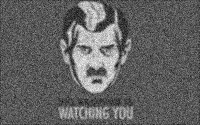
\includegraphics[width=0.3\textwidth]{./assets/1984_small_blur_noisy10.png}}
  &
  \raisebox{-0.5\height}{
\includegraphics[width=0.3\textwidth]{./assets/1984_small_reconstr_naive10.png}}
\end{tabular}
\end{center}

In order to better understand such a behaviour we will discuss it on a tiny \(2\times 2\) system of linear algebraic equations.
\begin{oppgave}
  Consider a \(2\times 2\) matrix \(A\) and a vector \(b \in \R^2\) given by
  \begin{equation}\label{eq:lindep}
    A = \begin{bmatrix*}[r]
    1 & 1 \\ 1 & 1+\epsilon
    \end{bmatrix*}
    \qquad\text{and}\qquad
    b = \begin{bmatrix*}[r]
    2 \\ 2+\delta
    \end{bmatrix*},
  \end{equation}
  where \(\epsilon\) and \(\delta\) are small numbers (close to 0).
  Note that this setup corresponds to the dataset \((t_1,y_1)=(1,2)\) and
  \((t_2,y_2)=(1+\epsilon,2+\delta)\) in question 1.
  \begin{punkt}
    Sketch the two vectors corresponding to the two columns of the matrix \(A\) in~\eqref{eq:lindep} in \(\R^2\) for \(\epsilon = 0.5\),
    \(\epsilon = 0.01\) and \(\epsilon = 0\).
    Discuss, in what way the columns of \(A\) become ``almost linearly dependent'' for small \(\epsilon\approx 0\).
  \end{punkt}

  \def\Functionone(#1){(#1)}
  \def\Functiontwo(#1){(1.5*(#1))}
  \def\Functionthree(#1){1.01*(#1)}

  \begin{align*}
    \begin{tikzpicture}
      \begin{axis}[
            axis y line=center,
            axis x line=middle, 
            axis on top=true,
            xmin=-0.2,
            xmax=1.2,
            ymin=-0.2,
            ymax=1.7,
            height=6.0cm,
            width=9.0cm,
            grid,
            xtick={0,0.2,...,1},
            ytick={0,0.2,...,1.5},
        ]
        \addplot [domain=0:1, samples=50, mark=none, ultra thick, blue] {\Functionone(x)};
        \addplot [domain=0:1, samples=50, mark=none, ultra thick, blue] {\Functiontwo(x)};
        \filldraw[blue] (1,1) circle (2pt) node[anchor=west]{(1,1)};
        \filldraw[blue] (1,1.5) circle (2pt) node[anchor=west]{(1,1.5)};
        %\draw[dashed, domain=0:1, smooth, variable=\x, blue] plot ({\x}, {\x*1.1});
        %\draw[dashed, domain=0:1, smooth, variable=\x, blue] plot ({\x}, {\x*1.2});
        %\draw[dashed, domain=0:1, smooth, variable=\x, blue] plot ({\x}, {\x*1.3});
        %\draw[dashed, domain=0:1, smooth, variable=\x, blue] plot ({\x}, {\x*1.4});
      \end{axis}
    \end{tikzpicture}
    \begin{tikzpicture}
      \begin{axis}[
            axis y line=center,
            axis x line=middle, 
            axis on top=true,
            xmin=-0.2,
            xmax=1.2,
            ymin=-0.2,
            ymax=1.7,
            height=6.0cm,
            width=9.0cm,
            grid,
            xtick={0,0.2,...,1},
            ytick={0,0.2,...,1.5},
        ]
        \addplot [domain=0:1, samples=50, mark=none, ultra thick, blue] {\Functionone(x)};
        \addplot [domain=0:1, samples=50, mark=none, ultra thick, blue] {\Functionthree(x)};
        \filldraw[blue] (1,1) circle (2pt) node[anchor=west]{(1,1)};
        \filldraw[blue] (1,1.01) circle (2pt) node[anchor=east]{(1,1.01)};
      \end{axis}
    \end{tikzpicture} \\
    \begin{tikzpicture}
      \begin{axis}[
            axis y line=center,
            axis x line=middle, 
            axis on top=true,
            xmin=-0.2,
            xmax=1.2,
            ymin=-0.2,
            ymax=1.7,
            height=8.0cm,
            width=12.0cm,
            grid,
            xtick={0,0.2,...,1},
            ytick={0,0.2,...,1.5},
        ]
        \addplot [domain=0:1, samples=50, mark=none, ultra thick, blue] {\Functionone(x)};
        \addplot [domain=0:1, samples=50, mark=none, ultra thick, blue] {\Functionone(x)};
        \filldraw[blue] (1,1) circle (2pt) node[anchor=west]{(1,1)};
        \filldraw[blue] (1,1) circle (2pt) node[anchor=east]{(1,1)};
      \end{axis}
    \end{tikzpicture}
  \end{align*}
  When $\epsilon$ gets close to 0, the two columns (1,1) and (1,1+$\epsilon$) would be equal and thereby linearly dependent because they would be \emph{almost} be each others multiple. Hence, when $\epsilon \to 0$ then the columns becomes “almost linearly dependent”.

  \begin{punkt}
    Use Gaussian elimination to solve the system \(Ax =b\) with \(A\),
    \(b\) given in~\eqref{eq:lindep}, assuming that \(\epsilon \neq 0\).
    Write down the expression for the solution \(x\) in terms of the parameters \(\epsilon\neq 0\) and \(\delta\).
  \end{punkt}
  \begin{align*}
    Ax=b \Longleftrightarrow
    \begin{bmatrix}
      1 & 1 & 2 \\
      1 & 1 + \epsilon & 2 + \delta
    \end{bmatrix}
    \sim
    \begin{bmatrix*}[r]
      1 & 1 & 2 \\
      0 & \epsilon & \delta
    \end{bmatrix*}
    \sim
    \begin{bmatrix*}[r]
      1 & 1 & 2 \\
      0 & 1 & \frac{\delta}{\epsilon}
    \end{bmatrix*}
    \sim
    \begin{bmatrix}
      1 & 0 & 2-\frac{\delta}{\epsilon} \\
      0 & 1 & \frac{\delta}{\epsilon}
    \end{bmatrix}
  \end{align*}

  The expression for the solution $x$ will therefore be:
  \begin{align*}
    x=\begin{pmatrix}
      2-\frac{\delta}{\epsilon} \\
      \frac{\delta}{\epsilon}
    \end{pmatrix}
    \text{ where }
    \epsilon \neq 0
  \end{align*}

  \begin{punkt}
    We will now interpret parameter \(\delta\) as a random measurement noise.
    Explain how even very small changes to \(\delta\) may lead to very large changes in the solution \(x\), provided that \(\epsilon\neq 0\) is close to zero.

    Hint: you can compare pairs of solutions corresponding to \(\delta = 0\) and \(\delta = 0.01\) for various values of \(\epsilon\neq 0\): \(\epsilon = 0.1\), \(\epsilon = 0.01\), \(\epsilon = 0.0001\).
  \end{punkt}

  The solution from 3.2 was $x=\begin{pmatrix}2-\frac{\delta}{\epsilon} \\\frac{\delta}{\epsilon}\end{pmatrix}$where $\epsilon \neq 0$. We will now replace $\epsilon$ and $\delta$ with the various values given the question.

  \begin{align*}
    \delta=0, \epsilon = 0.1:\mathbf{x}=\begin{pmatrix}2-\frac{0}{0.1} \\\frac{0}{0.1}\end{pmatrix}=\begin{pmatrix}2 \\0\end{pmatrix} \\
    \delta=0, \epsilon = 0.01:\mathbf{x}=\begin{pmatrix}2-\frac{0}{0.01} \\\frac{0}{0.01}\end{pmatrix}=\begin{pmatrix}2 \\0\end{pmatrix} \\
    \delta=0, \epsilon = 0.0001:\mathbf{x}=\begin{pmatrix}2-\frac{0}{0.0001} \\\frac{0}{0.0001}\end{pmatrix}=\begin{pmatrix}2 \\0\end{pmatrix} \\
    \delta=1, \epsilon = 0.1:\mathbf{x}=\begin{pmatrix}2-\frac{1}{0.1} \\\frac{1}{0.1}\end{pmatrix}=\begin{pmatrix}-8 \\10\end{pmatrix} \\
    \delta=1, \epsilon = 0.01:\mathbf{x}=\begin{pmatrix}2-\frac{0}{0.01} \\\frac{1}{0.01}\end{pmatrix}=\begin{pmatrix}-98 \\100\end{pmatrix} \\
    \delta=1, \epsilon = 0.0001:\mathbf{x}=\begin{pmatrix}2-\frac{1}{0.0001} \\\frac{1}{0.0001}\end{pmatrix}=\begin{pmatrix}-9998 \\10000\end{pmatrix}
  \end{align*}
  As we can see from these values of $x$, there is a big difference whether $\delta=0$ or $\delta=1$. The reason is because $\delta$ is being divided by $\epsilon$ which is very close to 0, causing $\frac{\delta}{\epsilon}$ to become a very large number.
\end{oppgave}


The phenomenon we have observed and discussed is known as the \emph{ill conditioning}: small changes in problem's data lead to large changes in the solution.
One standard approach to dealing with ill-conditioned linear systems is known as the Tikhonov regularization.
In this approach, we multiply both sides of the the ill-conditioned system \(A\vc(O) = \vc(\tilde{P})\) with \(A^T\), and then ``improve'' the matrix \(A^TA\) in the left hand side of the system by adding the identity matrix multiplied by a small regularization parameter \(\alpha>0\).
Thus we end up with the following system of linear algebraic equations
for computing the deblurred image \(O\):
\[
  [\alpha I + A^T A]\vc(O) = A^T\vc(\tilde{P}),
\]
where \(\alpha>0\) is a regularization parameter, and \(I\) is the identity matrix.\footnote{%
In block 3 of this course we will return to linear algebraic systems of this type.}
The results of deblurring based on Tikhonov-regularization are shown below.
\begin{center}
\begin{tabular}{llcc}
  & \(\alpha\) &Blurry, noisy image \(\tilde{P}\) & Tikhonov regularized reconstructed image \(O\)\\
  No noise & \(10^{-6}\) &
  \raisebox{-0.5\height}{
\includegraphics[width=0.3\textwidth]{./assets/1984_small_blur.png}}
  &
  \raisebox{-0.5\height}{
\includegraphics[width=0.3\textwidth]{./assets/1984_small_reconstr_Tikh0.png}}
  \\
  1\% noise & \(10^{-2}\) &
  \raisebox{-0.5\height}{
\includegraphics[width=0.3\textwidth]{./assets/1984_small_blur_noisy1.png}}
  &
  \raisebox{-0.5\height}{
\includegraphics[width=0.3\textwidth]{./assets/1984_small_reconstr_Tikh1.png}}
  \\
  10\% noise & \(0.3\) &
  \raisebox{-0.5\height}{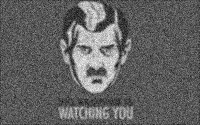
\includegraphics[width=0.3\textwidth]{./assets/1984_small_blur_noisy10.png}}
  &
  \raisebox{-0.5\height}{
\includegraphics[width=0.3\textwidth]{./assets/1984_small_reconstr_Tikh10.png}}
\end{tabular}
\end{center}

Two comments are in order.
\begin{itemize}
  \item Significanly better image deblurring algorithms exist. However, those go far beyond linear algebraic ideas, which we focus on in this course.
  \item Note that even for the small \(125\times 200\) image we consider in this workshop, the size of the algebraic system that we have to solve to reconstruct the image is \(n \times n = 25000\times 25000\).
  For a modestly sized image with \(768\times 1024\) pixels the algebraic system becomes \(786432\times 786432\) in size,
  and at 4K UHDTV resolution  of \(2160\times 3840\) we need to solve the system of the size \(8294400 \times 8294400\).
  Note that even to store all elements of the matrix (as 8-byte floating point numbers) for such a system would require \(8294400^2 \cdot 8 \text{B} \approx 500 GB\) of memory.

  Luckily, most elements of the matrix defining the system are zeros,
  and as such do not have to be stored.
  For solving such systems Gaussian elimination based algorithms quickly become inefficient or even infeasible.
  In the last part of this workshop we will discuss some simple alternative algorithms that may be used in place of Gaussian elimination for approximately solving systems of linear algebraic equations.
\end{itemize}

%------------------------------------------------------------------------
\section{Iterative algorithms for solving linear algebraic systems}

Whenever Gaussian elimination for solving linear algebraic systems is prohibitevely expensive, or simply inefficient, one can look at alternative approaches.
Unlike Gaussian elimination, which arrives at a solution to a linear system after performing a finite number of algorithmic steps, iterative algorithms construct an infinite sequence of vectors \(x^{(1)}, x^{(2)}, x^{(3)}, \dots\), which progressively become better and better approximations to  solution to the system of equations.

One of the simplest iterative algorithms for solving linear algebraic systems is the Gauss--Seidel method.
Consider the matrix equation \(Ax = b\), where
\[
  A =
  \begin{bmatrix*}[r]
    a_{1,1} & a_{1,2} & \dots & a_{1,n}\\
    a_{2,1} & a_{2,2} & \dots & a_{2,n}\\
    \vdots  & \vdots & \ddots &\vdots\\
    a_{n,1} & a_{n,2} & \dots & a_{n,n}
  \end{bmatrix*},
  \qquad
  x = \begin{bmatrix*}[r] x_1\\\vdots \\ x_n\end{bmatrix*},
  \quad
  \text{and}
  \quad
  b = \begin{bmatrix*}[r] b_1\\\vdots \\ b_n\end{bmatrix*}.
\]
We now split the matrix \(A\) into its lower triangle (including the diagonal)
\(L\) and the upper triangle \(U\):
\[
L =
\begin{bmatrix*}[r]
  a_{1,1} & 0 & \dots & 0\\
  a_{2,1} & a_{2,2} & \dots & 0\\
  \vdots  & \vdots & \ddots &\vdots\\
  a_{n,1} & a_{n,2} & \dots & a_{n,n}
\end{bmatrix*},
\qquad
\text{and}
\qquad
U = A-L =
\begin{bmatrix*}[r]
  0 & a_{1,2} & \dots & a_{1,n}\\
  0 & 0 & \dots & a_{2,n}\\
  \vdots  & \vdots & \ddots &\vdots\\
  0 & 0 & \dots & 0
\end{bmatrix*},
\]
and assume that all diagonal elements are non-zero: \(a_{i,i}\neq 0\), \(i=1,\dots,n\).
The algorithm is defined as follows.
\begin{algorithmic}[1]
\STATE Select some initial guess \(x^{(0)} \in \R^n\)
\FOR {\(k=0,1,2\dots\)}
  \STATE Solve the system
  \(L x^{(k+1)} = b - Ux^{(k)}\) to determine \(x^{(k+1)}\)
  \IF {\(x^{(k+1)} \approx x^{(k)}\) (up to some desired tolerance)}
    \STATE Stop, \(x^{(k+1)}\) is an approximate solution
    to the system \(Ax=b\)
  \ENDIF
\ENDFOR
\end{algorithmic}

We will now discuss a few basic details of this algorithm.
As a specific example, we will use a small \(4\times 4\) system
defined by
\begin{equation}\label{44}
  A = \begin{bmatrix*}[r]
  -12& 4& 0& -6\\
  6& 14& 3& -3\\
  -5& -8& 24& 8\\
  1& -4& 10& 16
  \end{bmatrix*}
  \qquad\text{and}\qquad
  b = \begin{bmatrix*}[r]-8\\47\\-93\\-13\end{bmatrix*}
\end{equation}
The behaviour of Gauss--Seidel algorithm for this (very small) system, starting from the initial guess \(x^{(0)} = [1,2,3,4]^T\), is illustrated in the figure below.
\begin{center}
  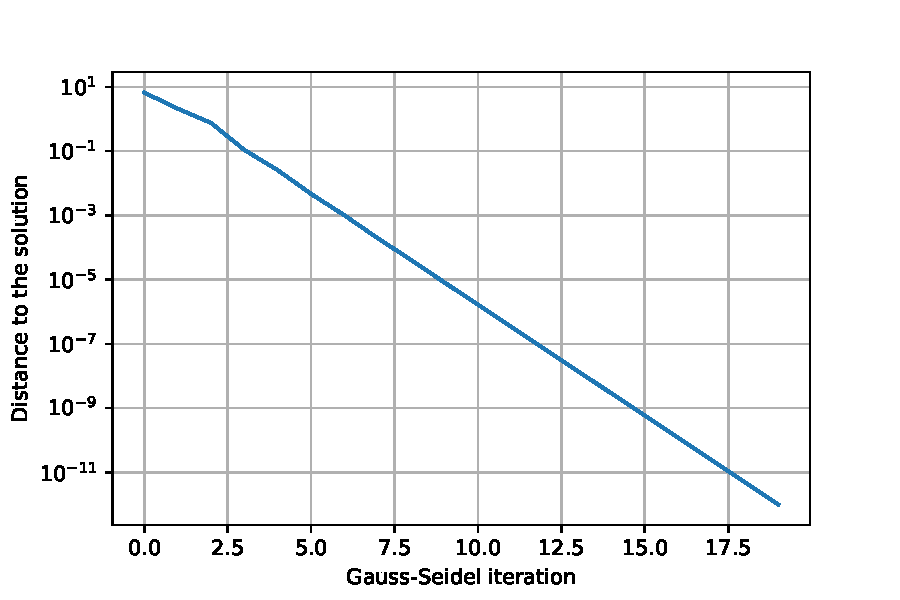
\includegraphics[width=0.5\textwidth]{./assets/gs44.pdf}
\end{center}
\begin{oppgave}
  \begin{punkt}
    Write down the matrices \(L\) and \(U\) corresponding to the system~\eqref{44}.
  \end{punkt}
  \begin{align*}
    L=\begin{bmatrix}
      -12 & 0 & 0 & 0 \\ 
      6 & 14 & 0 & 0 \\
      -5 & -8 & 24 & 0 \\
      1 & -4 & 10 & 16
    \end{bmatrix},
    U=\begin{bmatrix}
      0 & 4 & 0 & -6 \\ 
      0 & 0 & 3 & -3 \\
      0 & 0 & 0 & 8 \\
      0 & 0 & 0 & 0
    \end{bmatrix}
  \end{align*}

  \begin{punkt}
    Let \(x^{(0)} = [1,2,3,4]^T\).
    Compute the next iterate \(x^{(1)}\) in the Gauss--Seidel algorithm applied to the system~\eqref{44}.

    Note: in order to solve the system of linear algebraic equations on line 3 of the algorithm, one does not need to carry out Gaussian elimination.
    Note that one can compute \(x^{(1)}_1\) from the first equation in the system; with this knowledge, \(x^{(1)}_2\) can be computed using the second equation in the system, etc.
  \end{punkt}
  \begin{align*}
    x^{(0)}=[1,2,3,4]^T \\
    x^{(k+1)}=Lx^{(k+1)}=b-Ux^{(k)} \\
    x^{(1)}=Lx^{(1)}=b-Ux^{(0)} \\
    x^{(1)}=\begin{bmatrix}
      -12 & 0 & 0 & 0 \\ 
      6 & 14 & 0 & 0 \\
      -5 & -8 & 24 & 0 \\
      1 & -4 & 10 & 16
    \end{bmatrix}x^{(1)}=
    \begin{bmatrix}
      -8 \\ 47 \\ -93 \\ -13
    \end{bmatrix}
    -
    \begin{bmatrix}
      0 & 4 & 0 & -6 \\ 
      0 & 0 & 3 & -3 \\
      0 & 0 & 0 & 8 \\
      0 & 0 & 0 & 0
    \end{bmatrix}
    \begin{bmatrix}
      1 \\ 2 \\ 3 \\ 4
    \end{bmatrix} \\
    x_1^{(1)}:-12x_1=-8-(4(2)-6(4)) \Longleftrightarrow -12x_1=8 \Longleftrightarrow x_1=\frac{8}{-12} \Longleftrightarrow x_1=-0.\overline{66} \\
    x_2^{(2)}:6x_1+14x_2=50 \Longleftrightarrow x_2=\frac{-6(-0.\overline{66})+50}{14} \Longleftrightarrow x_2=3.85 \\ 
    x_3^{(3)}:-5x_1-8x_2+24x_3=-125 \Longleftrightarrow x_3=\frac{5(-0.\overline{66})+8(3.85)-125}{24}=x_3=-4.06 \\
    x_4^{(4)}:1x_1-4x_2+10x_3+16x_4=-13 \Longleftrightarrow x_4=\frac{-1(0.\overline{66})+4(3.85)-10(-4.06)-13}{16}=x_4=2.64 \\
    \text{\emph{Solution is therefore:}} \\
    x_1^{(1)}=-0.\overline{66},\;x_2^{(1)}=3.85,\;x_3^{(1)}=-4.06,\;x_4^{(1)}=2.64 \Longleftrightarrow x^{(1)}=\begin{pmatrix}-0,\overline{66} \\3.85 \\-4.06 \\2.64\end{pmatrix}
  \end{align*}

  \begin{punkt}
    Let now \(x^{(0)} = [1, 4, -3, 2]^T\).
    Show that the next iterate \(x^{(1)}\) in the Gauss--Seidel algorithm applied to the system~\eqref{44} equals \(x^{(0)}\).
    Does \(x^{(0)}\) solve the system~\eqref{44}?
  \end{punkt}
  \begin{align*}
    Lx^{(1)}=b-Ux^{(0)} \text{ We want to show that the next iterate } x^{(1)} \text{ equals } x^{(0)} \\
    Ux^{(0)}=\begin{bmatrix}0 & 4(4) & 0 & -6(2) \\0 & 0 & 3(-3) & -3(2) \\0 & 0 & 0 & 8(2) \\0 & 0 & 0 & 0\end{bmatrix}=\begin{bmatrix}4 \\-15 \\16 \\ 0\end{bmatrix} \\
    Lx^{(1)}=b-Ux^{(0)} \Longleftrightarrow \begin{bmatrix}-8 \\47 \\-93 \\-13\end{bmatrix}-\begin{bmatrix}4 \\-15 \\16 \\ 0\end{bmatrix}=\begin{bmatrix}-12 \\62 \\-109 \\-13\end{bmatrix} \\
    L=\begin{bmatrix}-12 & 0 & 0 & 0 \\6 & 14 & 0 & 0 \\-5 & -8 & 24 & 0 \\1 & -4 & 10 & 16\end{bmatrix}x^{(1)}=\begin{bmatrix}-12 \\62 \\-109 \\-13\end{bmatrix}\Longleftrightarrow\begin{bmatrix}-12 & 0 & 0 & 0 & -12\\6 & 14 & 0 & 0 & 62 \\-5 & -8 & 24 & 0 & -109 \\1 & -4 & 10 & 16 & -13\end{bmatrix} \\
    x_1^{(1)}=\frac{-12}{-12}=1 \\
    x_2^{(1)}=62-6(x_1)=62-6(1)=\frac{56}{14}=4 \\
    x_3^{(1)}=\frac{5(x_1)+8(x_2)-109}{24}=\frac{5(1)+8(4)-109}{24}=\frac{-72}{24}=-3 \\
    x_4^{(1)}=\frac{-1(x_1)+4(x_2)-10(x_3)-13}{16}=\frac{-1+4(4)-10(-3)-13}{16}=\frac{32}{16}=2 \\
    x^{(0)}=[1,4,-3,2]^T \\
    x^{(1)}=[1,4,-3,2]^T \\
    x^{(0)}=x^{(1)} \text{ Hence it is a solution}
  \end{align*}
  \textbf{Yes!} $x^{(0)}$ does solve the system (4) because line 4 in the algorithm is saying that if $x^{(k+1)} \approx x^{(k)} \Leftrightarrow x^{(1)} \approx x^{(0)}$ is true, then it is an approximate solution to the system, $Ax=b$. Because $x^{(1)} \approx x^{(0)}$ it does solve the system.
  \newline

  We will now generalize the observations in points 4.3 and 4.2.
  \begin{punkt}
    Assume that at some iteration \(k\) of the Gauss--Seidel algorithm
    we have that \(x^{(k+1)} = x^{(k)}\).
    Show that \(x^{(k)}\) solves the system \(Ax = b\).
    This explains the stopping criterion on line 4 of the Gauss--Seidel algorithm.
  \end{punkt}
  \begin{align*}
    Lx^{(k+1)}=b-Ux^{(k)} && \text{ Line 3 in algorithm}\\
    Lx^{(k)}=b-Ux^{(k)} && \text{ Assuming at some iteration $k$ that $x^{(k+1)}=x^{(k)}$}\\
    Lx^{(k)}+Ux^{(k)}=b \\
    (L+U)x^{(k)}=b && \text{ Distributive law} \\
    Ax^{(k)}=b && \text{ Given $A=L+U$}
  \end{align*}

  \begin{punkt}
    Explain why the following \emph{forward substitution} algorithm solves the system of linear algebraic equations $L x^{(k+1)} = b - Ux^{(k)}$ found on line 3 of the Gauss--Seidel algorithm:\\
    \begin{algorithmic}[1]
      \FOR {\(i=1,2,\dots,n\)}
        \STATE \[x^{(k+1)}_i = a_{i,i}^{-1}
        \left[b - \sum_{j=1}^{i-1} a_{i,j}x^{(k+1)}_j
        - \sum_{j=i+1}^{n} a_{i,j}x^{(k)}_j\right]\]
      \ENDFOR
    \end{algorithmic}
  \end{punkt}
  \begin{align*}
    Ux^{(k)}=\sum_{j=i+1}^{n} a_{i,j}x^{(k)}_j
  \end{align*}
  The equation can be rewritten as
  \begin{align*}
    Lx^{(k+1)}=b-Ux^{(k)} \Rightarrow x^{(k+1)}=L^{-1}(b-Ux^{(k)})
  \end{align*}
\end{oppgave}

\end{document}
